
%----------------------------------------------------------------------------------------
%	PACKAGES AND OTHER DOCUMENT CONFIGURATIONS
%----------------------------------------------------------------------------------------

\documentclass[twoside, column]{article}
% For two column: \documentclass[twoside, twocolumn]{article}

\usepackage{blindtext} % Package to generate dummy text throughout this template 

\usepackage[sc]{mathpazo} % Use the Palatino font
\usepackage[T1]{fontenc} % Use 8-bit encoding that has 256 glyphs
\linespread{1.05} % Line spacing - Palatino needs more space between lines
\usepackage{microtype} % Slightly tweak font spacing for aesthetics

\usepackage[english]{babel} % Language hyphenation and typographical rules

\usepackage[hmarginratio=1:1,top=32mm,columnsep=20pt]{geometry} % Document margins
\usepackage[hang, small,labelfont=bf,up,textfont=it,up]{caption} % Custom captions under/above floats in tables or figures
\usepackage{booktabs} % Horizontal rules in tables

\usepackage{lettrine} % The lettrine is the first enlarged letter at the beginning of the text

\usepackage{enumitem} % Customized lists
\setlist[itemize]{noitemsep} % Make itemize lists more compact

\usepackage{abstract} % Allows abstract customization
\renewcommand{\abstractnamefont}{\normalfont\bfseries} % Set the "Abstract" text to bold
\renewcommand{\abstracttextfont}{\normalfont\small\itshape} % Set the abstract itself to small italic text

\usepackage{titlesec} % Allows customization of titles
\renewcommand\thesection{\Roman{section}} % Roman numerals for the sections
\renewcommand\thesubsection{\roman{subsection}} % roman numerals for subsections
\titleformat{\section}[block]{\large\scshape\centering}{\thesection.}{1em}{} % Change the look of the section titles
\titleformat{\subsection}[block]{\large}{\thesubsection.}{1em}{} % Change the look of the section titles

\usepackage{fancyhdr} % Headers and footers
\pagestyle{fancy} % All pages have headers and footers
\fancyhead{} % Blank out the default header
\fancyfoot{} % Blank out the default footer
\fancyhead[C]{Multi-digit Prediction with Convolutional Neural Networks, Ritchie Ng, Version 1} % Custom header text
\fancyfoot[RO,LE]{\thepage} % Custom footer text

\usepackage{titling} % Customizing the title section

\usepackage{hyperref} % For hyperlinks in the PDF

\usepackage[utf8]{inputenc}
\usepackage{minted}

\usepackage{graphicx}
\graphicspath{ {images/} }


%----------------------------------------------------------------------------------------
%	TITLE SECTION
%----------------------------------------------------------------------------------------

\setlength{\droptitle}{-4\baselineskip} % Move the title up

\pretitle{\begin{center}\Huge\bfseries} % Article title formatting
\posttitle{\end{center}} % Article title closing formatting
\title{Large-scale Identification of Multiple Digits From Real-World Images with Convolutional Neural Networks} 
\author{%
\textsc{Ritchie Ng}\\ 
\normalsize National University of Singapore\\ 
\normalsize \href{mailto:ritchieng@u.nus.edu}{ritchieng@u.nus.edu} 
}
\date{\today} % Leave empty to omit a date
\renewcommand{\maketitlehookd}{%
\begin{abstract}
% Dummy abstract text - replace \blindtext with your abstract text
\noindent 
Convolutional Neural Networks (ConvNets) have been known to be effective in predicting digits as shown from the typical MNIST dataset. This project aims to predict multiple digits from Google's The Street View House Numbers (SVHN) dataset. A quick search online would show how this has not been thoroughly explored compared to other datasets like MNIST, CIFAR-10, CIFAR-100 and ImageNet. In particular, this project aims to provide the base for others to easily swap out the topology of the ConvNet, except the readout layers, to proven working topologies such as GoogLeNet, VGGNet and ResNet.
\end{abstract}
}

%----------------------------------------------------------------------------------------

\begin{document}

% Print the title
\maketitle

%----------------------------------------------------------------------------------------
%	ARTICLE CONTENTS
%----------------------------------------------------------------------------------------

\section{Introduction}

%------------------------------------------------

\subsection{Overview}
This project explores how convolutional neural networks (ConvNets) can be used to effectively identify a series of digits from real-world images that are obtained from \textit{The Street View House Numbers (SVHN) Dataset}.  ConvNets have evolved dramatically every year since the inception of the ImageNet Challenge in 2010. 

A proverbial ConvNet structure is the \textit{LeNet-5} that has relatively few layers of convolutions, poolings, and full connections. Subsequently, with the advent of the ImageNet Challenge, we are experiencing a gradual trend towards deeper ConvNets with more layers and higher accuracy such as \textit{AlexNet}, \textit{ZFNet}, \textit{VGGNet}, \textit{GoogLeNet}, and \textit{ResNet} being the latest state-of-the-art implementation of ConvNets.  

To this point, I started off with a simple ConvNet structure as a base where I made refinements to determine my optimal model for identifying multiple digits from real-world images.

%------------------------------------------------

\subsection{Problem Statement}
I am attempting to predict a series of numbers given an image of house numbers from the SVHN dataset. An important thing to take note is that instead of the standard identification of numbers, as with the MNIST dataset, I now need to correctly detect the numbers and the sequence of numbers. 

%------------------------------------------------

\subsection{Metric}

Across the models, I compared the training, validation and test accuracies. And accuracy is measured by Equation (1).

\begin{equation} \label{}
\frac{TP + TN}{TP + TN + FP + FN}
\end{equation}

Using Numpy, I created an accuracy function that is catered towards the problem of multi-digit prediction. 

\definecolor{bg}{rgb}{0.95,0.95,0.95}
\begin{minted}[bgcolor=bg]{python}
def accuracy(predictions, labels):
    return (100.0 * np.sum(np.argmax(predictions, 2).T == labels)
            / predictions.shape[1] / predictions.shape[0])      
 \end{minted}
 
%------------------------------------------------

\section{Analysis}

%------------------------------------------------
\subsection{Data Exploration}

There are 10 classes in the data, 1 for each digit and 10 denotes '0'. In total, there are 73257 digits for training, 26032 digits for testing, and 531131 extra digits. For my implementation, I used the raw images that came with a variety of dimensions as shown in Figure 1.

\begin{figure}[h]
\caption{Examples of the the database of raw images from SVHN}
\centering
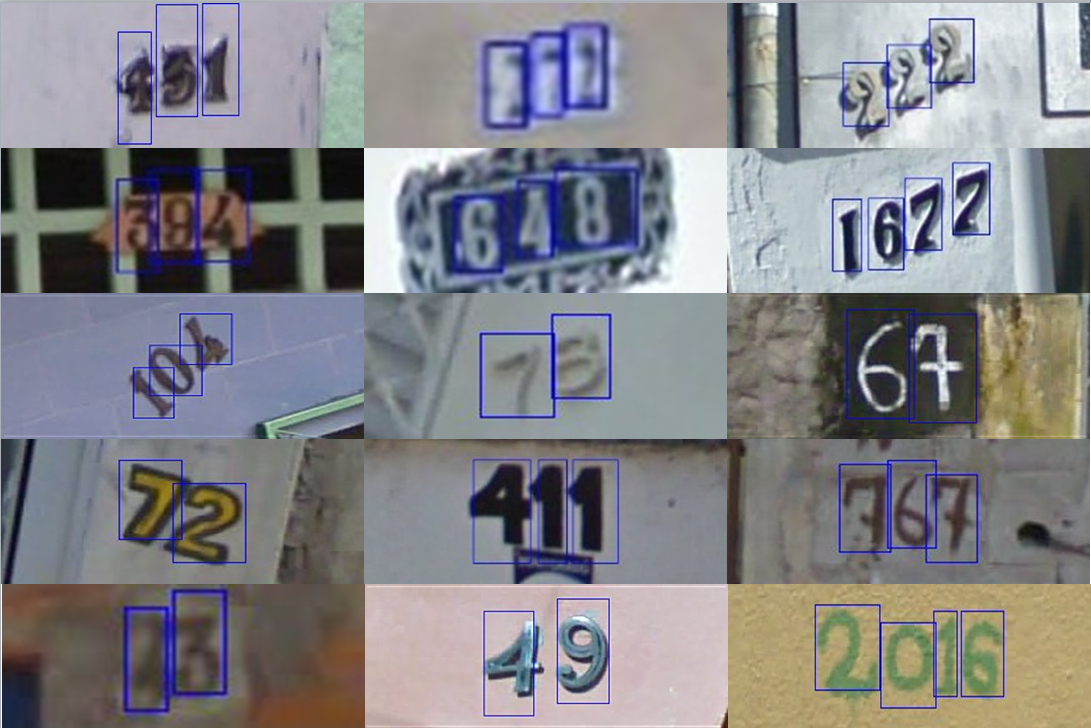
\includegraphics[width=0.5\textwidth]{original_photos}
\end{figure}

%------------------------------------------------
%	EXPLORATORY VISUALIZATIONS
\subsection{Exploratory Visualization}

When I went into the raw data to further explore the images, the images had a few properties as shown in Table 1. 

\begin{table}[htp]
\caption{Examining Training Images}
\begin{center}
\begin{tabular}{llr}

\cmidrule(r){1-2}
Image Number & Description \\
\midrule
141 & The image was barely perceptible even for a person.\\
180 & This is a typical clear image. \\
337 & This image has an "N" before the numbers. \\
645 & This image has multiple alphabets. \\
650 & This image has a confusing line amongst the numbers. \\

\end{tabular}
\end{center}
\label{default}
\end{table}

\begin{figure}
\caption{Blur image 141}
\centering
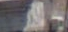
\includegraphics[width=0.5\textwidth]{141_blur}
\end{figure}

\begin{figure}
\caption{Clear image 180}
\centering
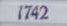
\includegraphics[width=0.5\textwidth]{180_clear}
\end{figure}

\begin{figure}
\caption{Image 337 with an alphabet}
\centering
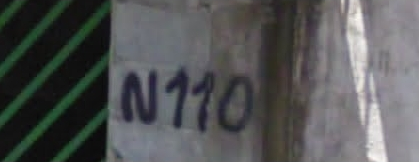
\includegraphics[width=0.5\textwidth]{337_alphabets}
\end{figure}

\begin{figure}
\caption{Image 645 with multiple alphabets}
\centering
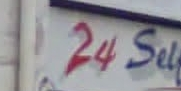
\includegraphics[width=0.5\textwidth]{645_alphabets}
\end{figure}

\begin{figure}
\caption{Image 650 with confusing line}
\centering
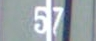
\includegraphics[width=0.5\textwidth]{650_confusing}
\end{figure}

Image 141 in Figure 2 may be an issue for the ConvNet to predict the correct numbers.  Likewise, images 337, 645 and 650 may have issues due to alphabets and confusing lines as shown in Figures 4, 5, and 6. On the other hand, image 180 from Figure 3 would be easy for the ConvNet to predict and fortunately the majority of images are similar to this. 

%------------------------------------------------
%	ALGORITHMS AND TECHNIQUES
\subsection{Algorithms and Techniques}

My programming language of choice is Python 2.7 and I will be using TensorFlow to build our deep ConvNets. Also, this project uses Tensorboard extensively for visualizations. It is a relatively new area for many people who are using Tensorflow and there are detailed instructions on how this has been implemented and how you can view the interactive visualizations in the implementations section.

Other substantial packages that are needed to run the code are shown in the following code snippet. Most of them are used for loading the data and processing the data. With $numpy$ being the most used package for data manipulation.

\definecolor{bg}{rgb}{0.95,0.95,0.95}
\begin{minted}[bgcolor=bg]{python}
import os
import sys
import tarfile
import tarfile
import tensorflow as tf
import numpy as np, h5py 
from __future__ import print_function
from six.moves import cPickle as pickle
from six.moves import range
from six.moves.urllib.request import urlretrieve
from scipy import ndimage
from PIL import Image
from numpy import random
 \end{minted}

The models' computations are accelerated with a CUDA-enabled GPU on Amazon Web Service (AWS) with a g2.2xlarge EC2 instance and a 60 GB EBS volume attached to it and each trial went through 60,000 steps to achieve the results reported. 

% Text requiring further explanation\footnote{Example footnote}.
% A statement requiring citation \cite{Figueredo:2009dg}.

%----------------------------------------------------------------------------------------

\subsection{Benchmark}

I compared test accuracies across the models to determine the best model. The higher the test accuracy, the better the model. And the model with the highest test accuracy is deemed as the best model. Validation and training accuracies are not considered for comparison because they are not as representative of the the model's predictive capability on unseen data. 

%----------------------------------------------------------------------------------------

\section{Methodology}

%----------------------------------------------------------------------------------------
%	DATA PREPROCESSING

\subsection{Data Preprocessing}

It is important to note that the images came in many dimensions. As such, I located the bounding boxes and cropped the images using the bounding boxes' location such that all images are of the size 32 x 32 pixels. Moreover, I also normalized the images and converted them from 3 channels, color images, to 1 channel, greyscale images. 

It is important to note that there were originally 73257 digits for training, 26032 digits for testing, and 531131 extra digits. I distributed the extra digits and testing digits randomly to increase our training dataset so I have more data to train on. Moreover, I deleted an image that had more than 5 digits as it is an anomaly in the training set. The final shapes of the datasets' tensors and labels' arrays are shown in the following code snippet.

\definecolor{bg}{rgb}{0.95,0.95,0.95}
\begin{minted}[bgcolor=bg]{python}
Training data shape: (230070, 32, 32, 1)
Training label shape: (230070, 6)
Validation data shape: (5684, 32, 32, 1)
Validation label shape: (5684, 6)
Test data shape: (13068, 32, 32, 1)
Test label shape: (13068, 6)
 \end{minted}
 
 All the processed images are then pickled into a file named SVHN.pickle where anyone can easily access through the following code. 
 
\definecolor{bg}{rgb}{0.95,0.95,0.95}
\begin{minted}[bgcolor=bg]{python}
print('Loading pickled data...')

pickle_file = 'SVHN.pickle'

with open(pickle_file, 'rb') as f:
    save = pickle.load(f)
    X_train = save['train_dataset']
    y_train = save['train_labels']
    X_val = save['valid_dataset']
    y_val = save['valid_labels']
    X_test = save['test_dataset']
    y_test = save['test_labels']
    del save  
    print('Training data shape:', X_train.shape)
    print('Training label shape:',y_train.shape)
    print('Validation data shape:', X_val.shape)
    print('Validation label shape:', y_val.shape)
    print('Test data shape:', X_test.shape)
    print('Test label shape:', y_test.shape)
    
print('Data successfully loaded!')
 \end{minted}
 
 %----------------------------------------------------------------------------------------

%	TRIAL 1
\subsection{Implementation of Trial 1}

In this first trial, I started off with a simple model comprising the following layers. 

\begin{table}[htp]
\caption{ConvNet Topology: Trial 1}
\begin{center}
\begin{tabular}{llr}

\cmidrule(r){1-2}
Layer & Description \\
\midrule
Input Layer & Numpy array of size (230070, 32, 32, 1)\\
Convolution 1 & Filters: 16 | Receptive Field: 5 x 5 | Stride: 2 | Padding: Valid\\
ReLU & Rectified Linear Unit Activation\\
Max Pooling & Receptive Field: 2 x 2 | Stride: 2 | Padding: Valid\\
Convolution 2 & Filters: 32 | Receptive Field: 5 x 5 | Stride: 2 | Padding: Valid\\
ReLU & Rectified Linear Unit Activation\\
Max Pooling & Receptive Field: 2 x 2 | Stride: 2 | Padding: Valid\\
Convolution 3 & Filters: 96 | Receptive Field: 5 x 5 | Stride: 2 | Padding: Valid\\
ReLU & Rectified Linear Unit Activation\\
Dropout & Keep probability of 0.5\\
Fully Connected Layer (FC) & Nodes: 64\\
Softmax Layer & 5 softmax (readout) activation layers for 5 digits\\

\end{tabular}
\end{center}
\label{default}
\end{table}

As you can see from Figure 7, we have 3 convolution layers with 3 sets of weights and biases. And the final convolution layer feeds to the fully connected layer as seen in Figure 8.

\begin{figure}
\caption{Trial 1 Convolution Layers}
\centering
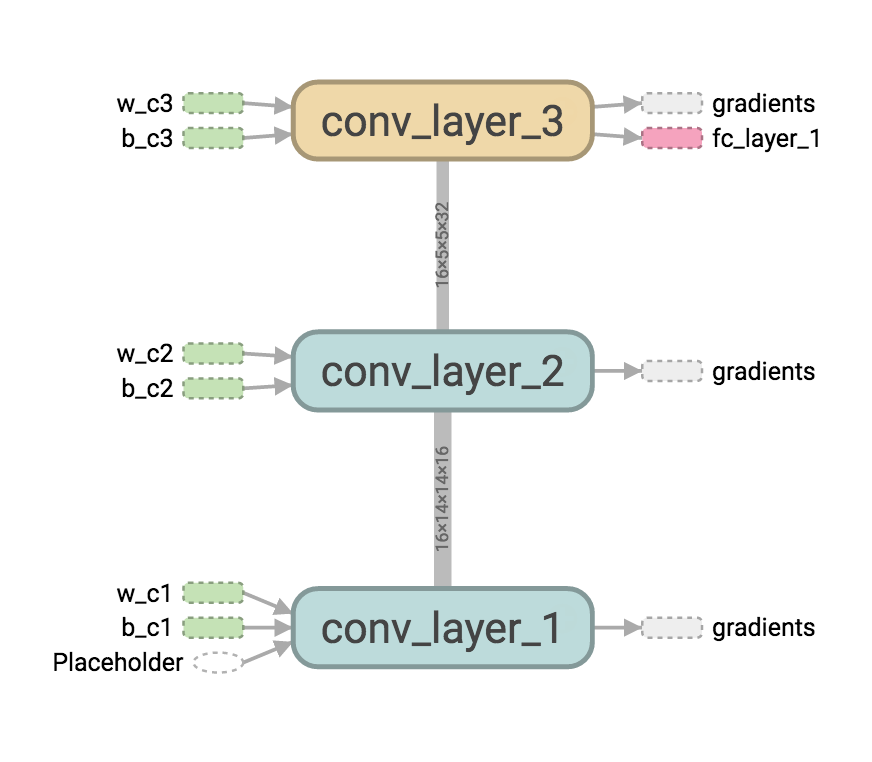
\includegraphics[width=0.5\textwidth]{conv_trial_1}
\end{figure}

\begin{figure}
\caption{Trial 1 FC Layer}
\centering
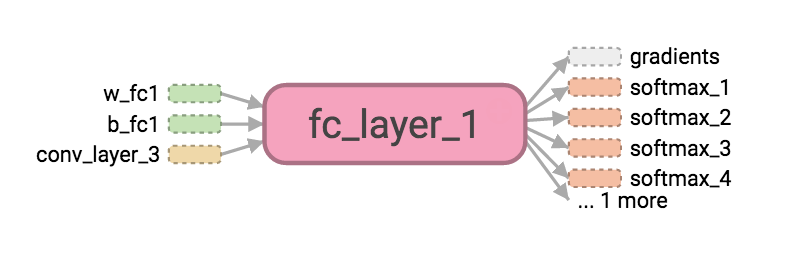
\includegraphics[width=0.5\textwidth]{fc_trial_1}
\end{figure}

Moreover, the weights are initialized with special functions I created so it is easier to expand the convolutional networks and have access to Tensorboard's visualizations. The weights are initialized with a random normal distribution with a standard deviation of 0.01. And the functions take in two arguments: the tensor and the names for Tensorboard's visualizations.
\definecolor{bg}{rgb}{0.95,0.95,0.95}
\begin{minted}[bgcolor=bg]{python}
    def init_weights(shape, name):
        return tf.Variable(
            tf.random_normal(shape=shape, stddev=0.01),
            name=name)

    def init_biases(shape, name):
        return tf.Variable(
            tf.constant(1.0, shape=shape),
            name=name
        )
\end{minted}
 
For my optimizer, I used Stochastic Gradient Descent (SGD) with a step-wise decay with a starting learning rate of 0.05. In the equation, I used step-wise decay, so $\frac {globalstep}{decaysteps}$ would return an integer. And in Figure 9, we can see the SGD's graph with the relevant weights and biases.
\begin{equation} \label{}
decayed learning rate = learningrate * decayrate^\frac{globalstep}{decaysteps}
\end{equation}

\begin{figure}
\caption{SGD Tensorboard graph}
\centering
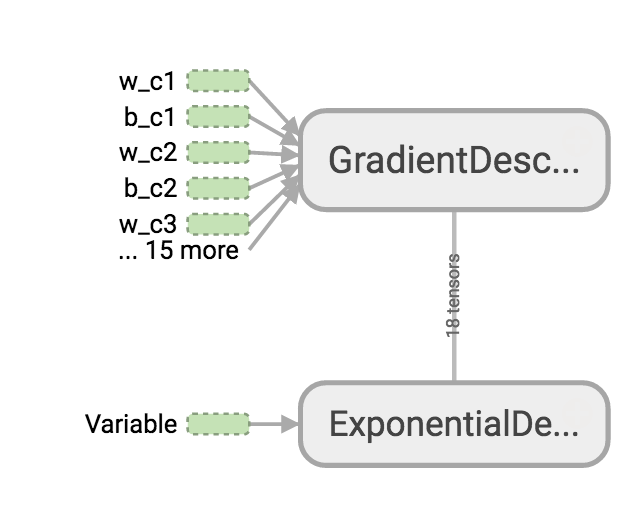
\includegraphics[width=0.5\textwidth]{gd_trial_1}
\end{figure}

Importantly, unlike running a ConvNet on the MNIST dataset or majority of the datasets, our loss function is a combination of the parallel softmax (readout) activation layers. The code of the loss function can be seen in the following code and the graphical representation can be seen in Figure 10.
\definecolor{bg}{rgb}{0.95,0.95,0.95}
\begin{minted}[bgcolor=bg]{python}
    with tf.name_scope("loss"):
        loss = tf.reduce_mean(tf.nn.sparse_softmax_cross_entropy_with_logits(
                   logits_1, tf_train_labels[:, 1])) + \
               tf.reduce_mean(tf.nn.sparse_softmax_cross_entropy_with_logits(
                   logits_2, tf_train_labels[:, 2])) + \
               tf.reduce_mean(tf.nn.sparse_softmax_cross_entropy_with_logits(
                   logits_3, tf_train_labels[:, 3])) + \
               tf.reduce_mean(tf.nn.sparse_softmax_cross_entropy_with_logits(
                   logits_4, tf_train_labels[:, 4])) + \
               tf.reduce_mean(tf.nn.sparse_softmax_cross_entropy_with_logits(
                   logits_5, tf_train_labels[:, 5]))
        # Add scalar summary for cost
        tf.scalar_summary("loss", loss)
 \end{minted}
 
\begin{figure}
\caption{Loss Tensorboard graph}
\centering
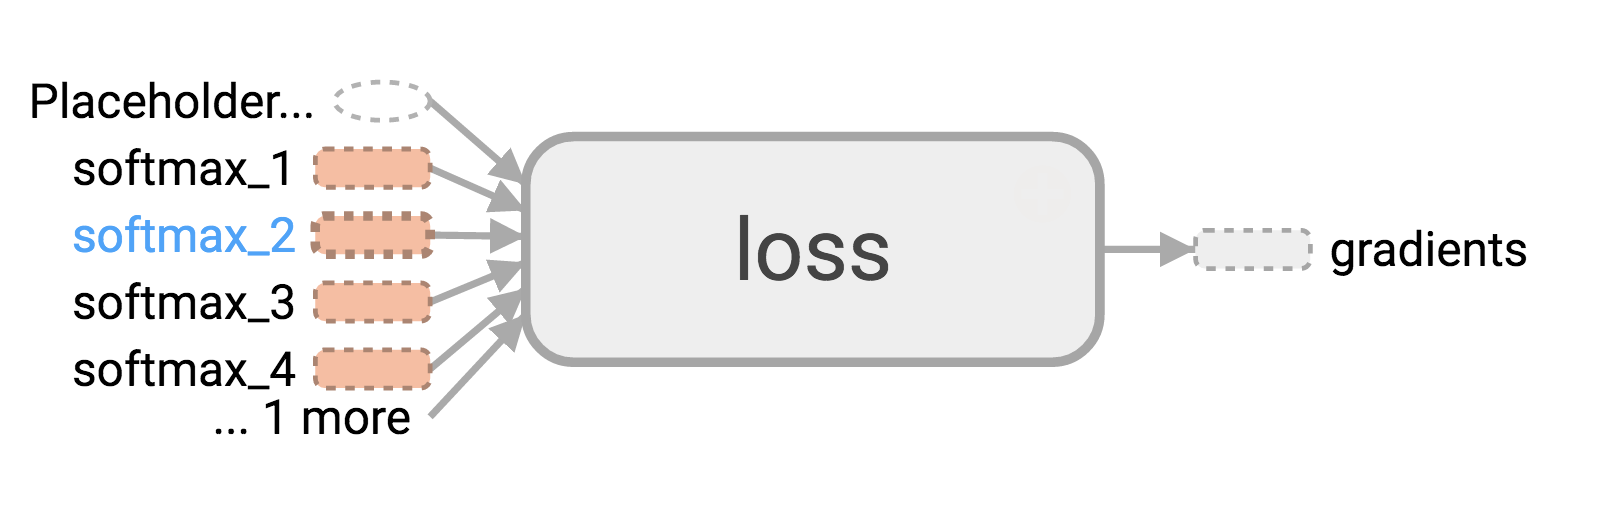
\includegraphics[width=0.5\textwidth]{loss_trial_2}
\end{figure}

With this model, I managed to achieve a test accuracy of 87.64\% and the training and validation accuracies are shown below. And it is interesting to note how the loss seems to plateau and they are very erratic as seen in Figure 11. 
\definecolor{bg}{rgb}{0.95,0.95,0.95}
\begin{minted}[bgcolor=bg]{python}
Minibatch accuracy: 90.0%
Validation accuracy: 87.2202674173%
Test accuracy: 87.6400367309%
 \end{minted}

\begin{figure}
\caption{Loss Tensorboard graph}
\centering
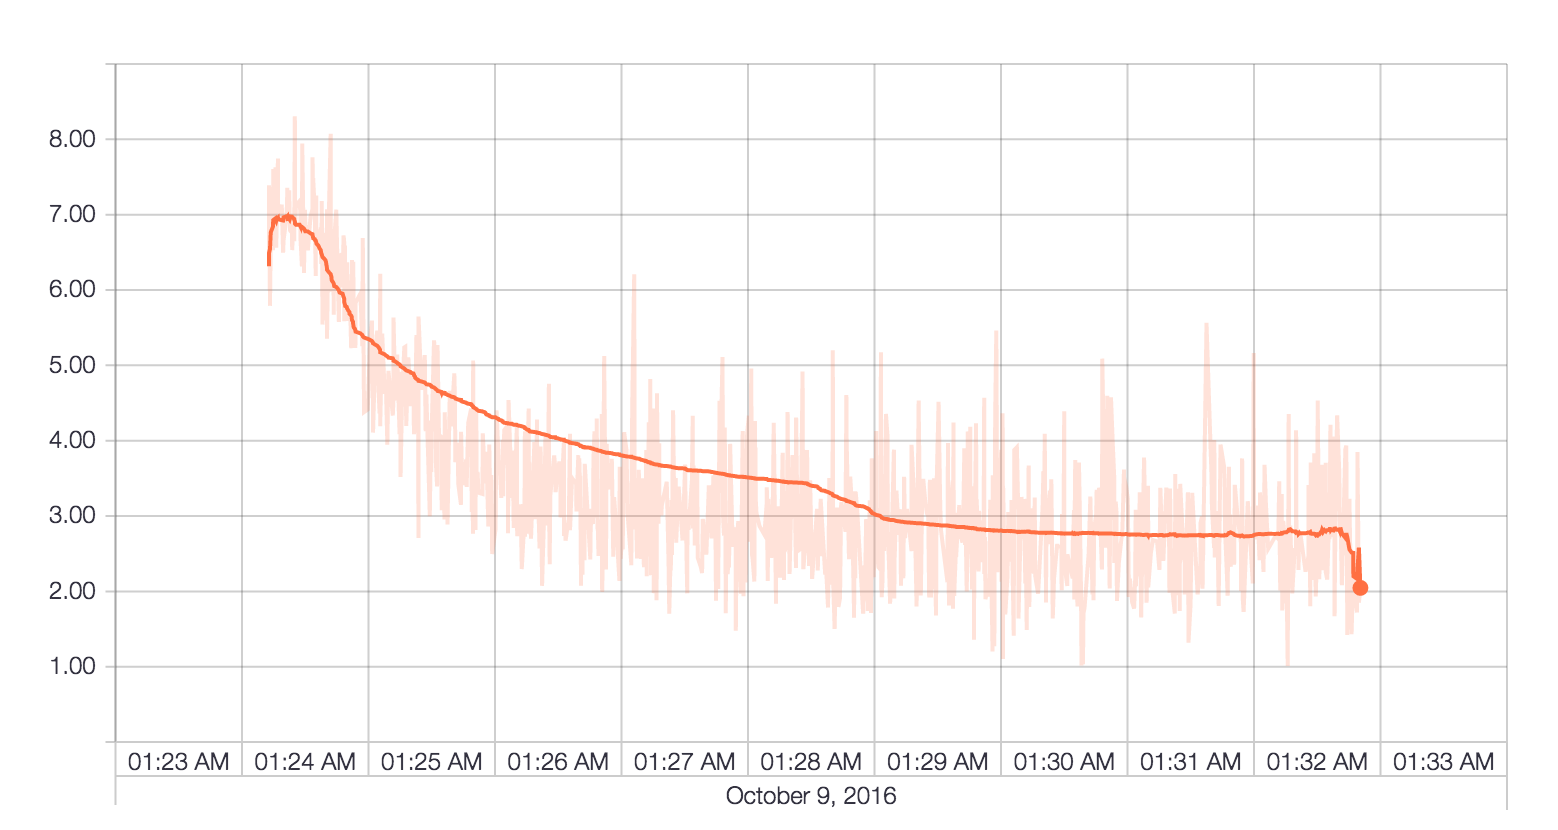
\includegraphics[width=0.5\textwidth]{loss_trial_1}
\end{figure}

I believe this warrants a second trial to refine some hyperparameters like my optimizer, initialization of weights, and the dropout probability. 

%----------------------------------------------------------------------------------------
 %	REFINEMENTS: TRIAL 2
 
 \subsection{Refinements}
 
In this section, I implemented our ConvNet with different hyperparameters from my first trial.
 
First, I changed my dropout probability to 0.8 and all else are similar as shown in Table 3. 

\begin{table}[htp]
\caption{ConvNet Topology: Trial 2}
\begin{center}
\begin{tabular}{llr}

\cmidrule(r){1-2}
Layer & Description \\
\midrule
Input Layer & Numpy array of size (230070, 32, 32, 1)\\
Convolution 1 & Filters: 16 | Receptive Field: 5 x 5 | Stride: 2 | Padding: Valid\\
ReLU & Rectified Linear Unit Activation\\
Max Pooling & Receptive Field: 2 x 2 | Stride: 2 | Padding: Valid\\
Convolution 2 & Filters: 32 | Receptive Field: 5 x 5 | Stride: 2 | Padding: Valid\\
ReLU & Rectified Linear Unit Activation\\
Max Pooling & Receptive Field: 2 x 2 | Stride: 2 | Padding: Valid\\
Convolution 3 & Filters: 96 | Receptive Field: 5 x 5 | Stride: 2 | Padding: Valid\\
ReLU & Rectified Linear Unit Activation\\
Dropout & Keep probability of 0.5\\
Fully Connected Layer (FC) & Nodes: 64\\
Softmax Layer & 5 softmax (readout) activation layers for 5 digits \\

\end{tabular}
\end{center}
\label{default}
\end{table}

Second, I changed my optimizer from SGD to AdaGrad. This is because our data is quick sparse for digits with many numbers and AdaGrad is well-suited for such a dataset because it adapts the learning rate to the parameters performing larger updates for infrequent parameters and smaller updates for frequent parameters.

Third, I changed the initialization of the weights using Xavier Initialization. It is a sampling of Gaussian distribution where the variance is a function of the number of neurons as shown in the following custom functions I made where the first function is for initializing weights for the convolution layers and the second function is for the initialization of weights for the FC layer after all the convolutions.

\definecolor{bg}{rgb}{0.95,0.95,0.95}
\begin{minted}[bgcolor=bg]{python}
    def init_weights_conv(shape, name):
        return tf.get_variable(shape=shape, name=name,
            initializer=tf.contrib.layers.xavier_initializer_conv2d())
    def init_weights_fc(shape, name):
        return tf.get_variable(shape=shape, name=name,
            initializer=tf.contrib.layers.xavier_initializer())
 \end{minted}
 
 With this, I managed to get a test accuracy of 91.62\% with the following test and validation accuracies.
 \definecolor{bg}{rgb}{0.95,0.95,0.95}
\begin{minted}[bgcolor=bg]{python}
Minibatch accuracy: 96.25%
Validation accuracy: 90.5594651654%
Test accuracy: 91.6176920722%
 \end{minted}
 
 Interestingly, unlikely previously the loss function is not plateauing and there seem to be more room for learning as shown on Figure 12.
 
\begin{figure}
\caption{Loss Tensorboard graph for Trial 2}
\centering
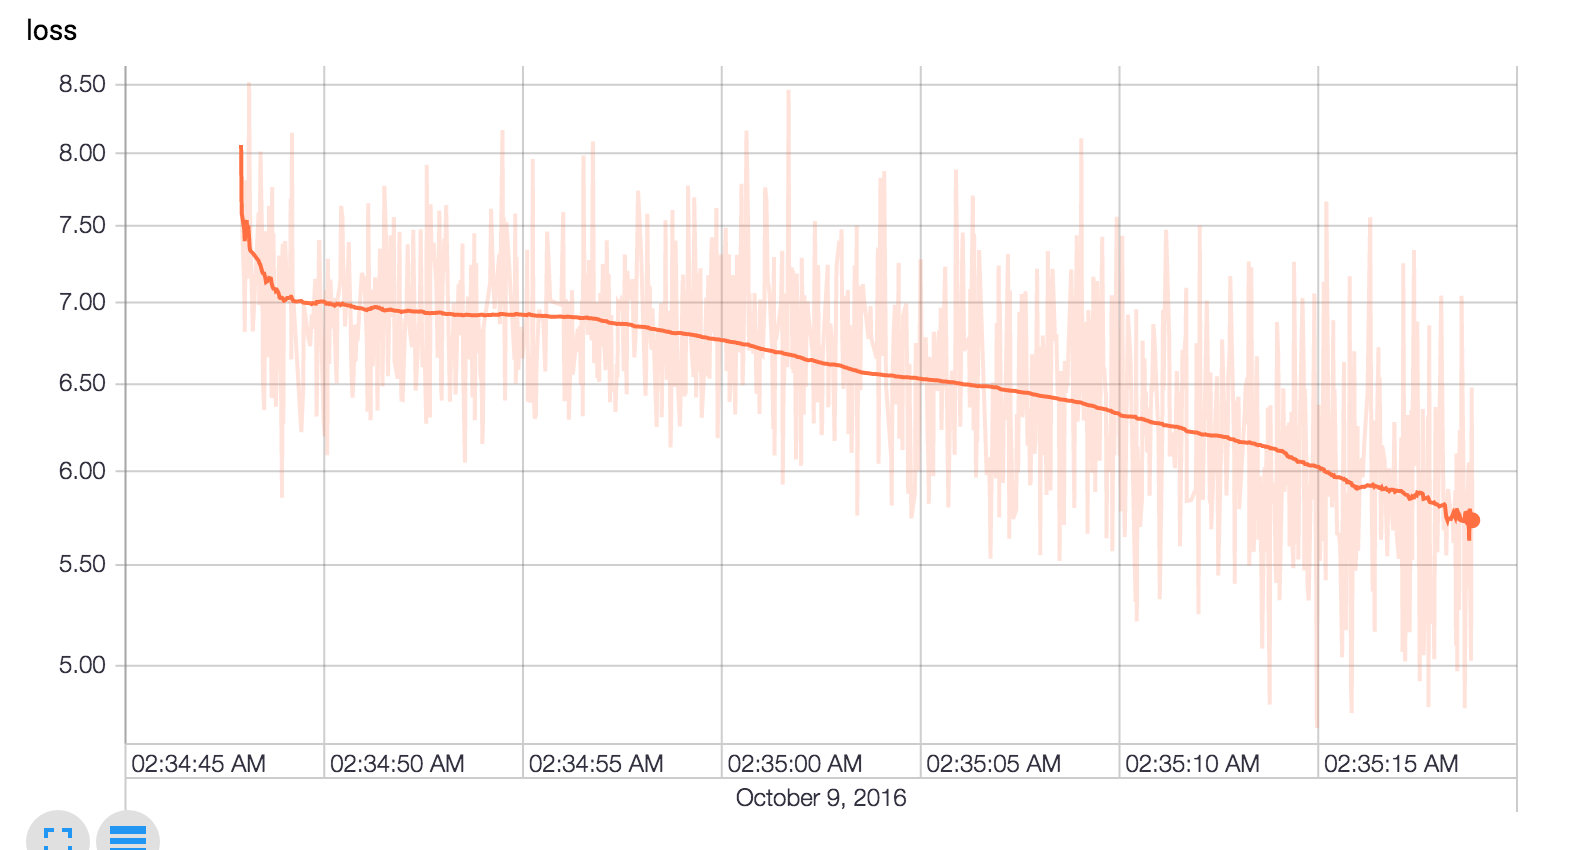
\includegraphics[width=0.5\textwidth]{trial_2_loss}
\end{figure}

%----------------------------------------------------------------------------------------
%	FINAL RESULTS
\section{Results}
 
 Comparing the two trials, we can see how the second model has a higher test accuracy and has yet to fully converged even with a higher accuracy. Moreover, the second model have higher validation and training accuracies too from Table 4 although we are not using them as a benchmark to decide the best model. Hence, since the second model has the best accuracy, I have decided to settle with this simple ConvNet that produced a respectable 91.62\% on unseen data.
 
 \begin{table}[htp]
\caption{Comparison of the performance of my models}
\begin{center}
\begin{tabular}{llr}

\cmidrule(r){1-3}
& Trial 1 & Trial 2 \\
\midrule
Test Accuracy  & 87.64\% & 91.62\%\\
Training Accuracy & 90.00\% & 96.25\% \\
Validation Accuracy &  87.22\% & 90.56\% \\

\end{tabular}
\end{center}
\label{default}
\end{table}
 
\subsection{Model Evaluation and Justification}
The huge performance gain from the second trial came from a more suitable optimizer, AdaGrad, compared to SGD due to the nature of our sparse data where we have few images with many digits like 4 or 5. Also, the initialization of the weights using Xavier's initializations contributed to this performance gain too. 


%----------------------------------------------------------------------------------------
%	CONCLUSION

\section{Conclusion}

The accuracy of the second model can be further improved with more training as it has yet to converge. Also, more investigation can be done to look at the large variation in our loss function. I did not use any renowned topology highlighted in the introduction such as $VGGNet$ or $ResNet$ to keep this project focused on how to classify multiple digits. This particular classification of multiple objects in a single image is lacking in examples online hence it provides a base for people to explore how we can use proven topologies such as $ResNet$ on this problem while maintaining the parallel readout layers to classify multiple digits. More importantly, there is room for improvement by using existing weights trained on the ImageNet dataset using $ResNet$ or other winning topologies and change the readout layer to the parallel readout layers. This may give a substantial boost to our test accuracy and reduce our training time. This method is recently coined as transfer learning and can be explored using this project's base code\footnote{You can access the open-source source code at https://github.com/ritchieng/NumNum.}.

%----------------------------------------------------------------------------------------
%	REFERENCE LIST
%----------------------------------------------------------------------------------------
%----------------------------------------------------------------------------------------

\end{document}
